\documentclass[10pt,landscape]{article}
\usepackage{multicol}
\usepackage{calc}
\usepackage{ifthen}
\usepackage[landscape]{geometry}
\usepackage{amsmath,amsthm,amsfonts,amssymb,courier}
\usepackage{color,graphicx,overpic}
\usepackage{hyperref}


\pdfinfo{
  /Title (example.pdf)
  /Creator (TeX)
  /Producer (pdfTeX 1.40.0)
  /Author (Seamus)
  /Subject (Example)
  /Keywords (pdflatex, latex,pdftex,tex)}

% This sets page margins to .5 inch if using letter paper, and to 1cm
% if using A4 paper. (This probably isn't strictly necessary.)
% If using another size paper, use default 1cm margins.
\ifthenelse{\lengthtest { \paperwidth = 11in}}
    { \geometry{top=.5in,left=.5in,right=.5in,bottom=.5in} }
    {\ifthenelse{ \lengthtest{ \paperwidth = 297mm}}
        {\geometry{top=1cm,left=1cm,right=1cm,bottom=1cm} }
        {\geometry{top=1cm,left=1cm,right=1cm,bottom=1cm} }
    }

% Turn off header and footer
\pagestyle{empty}

% Redefine section commands to use less space
\makeatletter
\renewcommand{\section}{\@startsection{section}{1}{0mm}%
                                {-1ex plus -.5ex minus -.2ex}%
                                {0.5ex plus .2ex}%x
                                {\normalfont\large\bfseries}}
\renewcommand{\subsection}{\@startsection{subsection}{2}{0mm}%
                                {-1explus -.5ex minus -.2ex}%
                                {0.5ex plus .2ex}%
                                {\normalfont\normalsize\bfseries}}
\renewcommand{\subsubsection}{\@startsection{subsubsection}{3}{0mm}%
                                {-1ex plus -.5ex minus -.2ex}%
                                {1ex plus .2ex}%
                                {\normalfont\small\bfseries}}
\makeatother

% Define BibTeX command
\def\BibTeX{{\rm B\kern-.05em{\sc i\kern-.025em b}\kern-.08em
    T\kern-.1667em\lower.7ex\hbox{E}\kern-.125emX}}

% Don't print section numbers
\setcounter{secnumdepth}{0}


\setlength{\parindent}{0pt}
\setlength{\parskip}{0pt plus 0.5ex}

%My Environments
\newtheorem{example}[section]{Example}
% -----------------------------------------------------------------------

\begin{document}
\raggedright
\footnotesize
\begin{multicols}{3}


% multicol parameters
% These lengths are set only within the two main columns
%\setlength{\columnseprule}{0.25pt}
\setlength{\premulticols}{1pt}
\setlength{\postmulticols}{1pt}
\setlength{\multicolsep}{1pt}
\setlength{\columnsep}{2pt}

%\begin{center}
%     \Large{\underline{CS 61C}} \\
%\end{center}

\subsection{Modular Arithmetic}
\hspace{5pt} $\cdot$ Addition: O(n)\\
\hspace{5pt} $\cdot$ Multiplication: O(n$^{2}$) {\it (naive)}\\
\hspace{5pt} $\cdot$ Multiplication: O(nlogn) {\it (FFT)}\\
\hspace{5pt} $\cdot$ Euclid's Rule: gcd(x, y) = gcd(x mod y, y)\\
\hspace{5pt} $\cdot$ \# of bits in x$^{y}$ = ylog$_{2}$x $\leq$ n$\cdot$2$^{n}$ \\
\vspace{1pt}\hspace{5pt} $\cdot$ $\frac{n}{2}^{\frac{n}{2}} \leq n! \leq n^{n}$\\
\vspace{1pt}\hspace{5pt} $\cdot$ {\it f:} S $\rightarrow$ T {\scriptsize is 1-to-1 (injective) \& onto (surjective) $\Rightarrow$ $\mid S \mid = \mid T \mid$}\\
\hspace{5pt} $\cdot$ {\it f:} S $\rightarrow$ T is 1-to-1 (injective) $\Rightarrow$ $\mid T \mid \geq \mid S \mid$\\
\hspace{5pt} $\cdot$ $\sum_{i=0}^{\infty}$ r$^{i}$ = $\frac{1}{1-r}$, if r $\textless$ 1\\
\hspace{5pt} $\cdot$ $\sum_{i=0}^{n}$ i$^{2}$ = $\frac{n(n+1)(2n+1)}{6}$\\
\hspace{5pt} $\cdot$ $\sum_{i=0}^{n}$ $\frac{1}{i}$ = O(log$_{2}$n)\\

\subsubsection{Extended Euclid's GCD(x,y)}
O(n$^{3}$); gcd(x,y) = d = x{\it i} + y{\it b}; x $\geq$ y; \# mod x\\
 \texttt{ext-gcd(x,y):\\ if y == 0: return (x, 1, 0)\\ else:\\ \hspace{3pt} (d, a, b) = ext-gcd(y, x mod y)\\\hspace{3pt} return (d, b, a-$\frac{x}{y}\cdot b$)}
 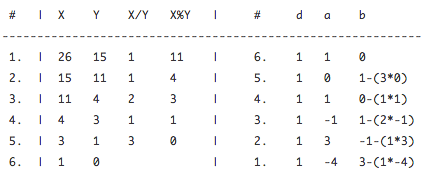
\includegraphics[scale=.45]{gcd.png}
 
 \subsubsection{Fermat's Little Theorem}
 if p is prime, then $\forall$ 1 $\leq$ a $\textless$ p\\
\hspace{5pt} a$^{p-1}$ = 1 mod p \\
\textit{\textbf{Proof:}}{\it Start by listing first p-1 positive multiples of a:\\
S = \{a, 2a, 3a, $\cdots$ (p -1)a\}\\
Suppose that {\it r}a and {\it s}a are the same mod p, $\Rightarrow$ {\it r = s} mod p\\
$\therefore$ set S of p-1 multiples of a are distinct and nonzero, that is, they must be congruent to 1, 2, 3, $\cdots$ p-1 after being sorted.\\
Multiply all congruences together and we find
a$\cdot$2a$\cdot$3a$\cdots$(p-1)$\cdot$a = 1$\cdot$2$\cdot$3$\cdots$(p-1) (mod p)
or better, a$^{(p-1)}$(p-1)! = (p-1)! mod p. Divide both side by (p-1)! $\blacksquare$}\\

\subsubsection{Primality Testing}
\begin{flushleft}\vspace{-16pt}\[
\hspace{-50pt}any \ a  \rightarrow a^{N-1} = 1 \ mod \ N {\it ?}
\begin{cases}
	{\it yes} \Rightarrow {\it "prime"}\\
	{\it no} \Rightarrow {\it composite}
\end{cases}
\]
\end{flushleft}
\vspace{-10pt}if N is not prime a$^{N-1}$ = 1 mod N $\leq$ half values of a $\textless$ N

\subsubsection{Lagrange's Prime Theorem}
Let $\pi$(x) be the \# of primes $leq$ x, then\\
$\pi$(x) $\approx$ $\frac{x}{ln(x)}$, or more precisely lim$_{x \rightarrow \infty} \frac{\pi(x)}{(\frac{x}{ln(x)})} = 1$\\

\subsubsection{Modular Exponentiation}
x$^{y}$ mod N $\rightarrow$ start with repeated squaring mod N\\
x mod N $\rightarrow$ x$^{2}$ mod N $\rightarrow$ (x$^{2}$)$^{^{2}}$ $\cdots$ x$^{log_{2}y}$ mod N\\
each step takes O(log$^{2}N)$ times to compute and \\there are log$_{2}$y steps, $\therefore$ $\in$ O(n$^{3}$),\\ where n is the \# of bits in N

\subsubsection{Formal Limit Proof}
\begin{flushleft}\vspace{-10pt}\[
\hspace{-50pt}lim_{n \rightarrow \infty}\frac{f(n)}{g(n)}
\begin{cases}
\hspace{3pt} \geq \ 0 \ {\it (\infty)} \Rightarrow \ f(n) \ \in \ \Omega(g(n))\\
\hspace{3pt} \textless \ \infty \ {\it (0)} \Rightarrow \ f(n) \ \in \ O(g(n))\\
\hspace{3pt} = c_{_{\mid 0 \textless c \textless \infty}} \Rightarrow \ f(n) \ \in \ \Theta(g(n))\\
\end{cases}
\]
\end{flushleft}

\subsubsection{Logarithm Tricks}
log$_{b}x^{p} = plog_{b}x$\\
$\frac{ln(x)}{ln(m)}$ = log$_{m}$x\\
x$^{log_{b}y} = y^{log_{b}x}$\\

\subsubsection{Complexity}
\hspace{3pt} $\cdot$ {\it f} $\in$ O({\it g}) if {\it f} $\leq$ c$\cdot${\it g}\\
\hspace{3pt} $\cdot$ {\it f} $\in$ $\Omega$({\it g}) if {\it f} $\geq$ c$\cdot${\it g}\\
\hspace{3pt} $\cdot$ {\it f} $\in$ $\Theta$({\it g}) if {\it f} $\in$ O({\it g}) \& $\Omega$({\it g})\\\vspace{1pt}
{\scriptsize \textit{{\vspace{1pt}Hierarchy:}}\\
\hspace{3pt} $\cdot$ Exponential\\
\hspace{3pt} $\cdot$ Polynomial\\
\hspace{3pt} $\cdot$ Logarithmic\\
\hspace{3pt} $\cdot$ Constant}\\


\subsubsection{Master's Theorem}
T(n) = aT($\frac{n}{b}$) + O(n$^{d}$), if a $\textgreater0, b\textgreater 1, d \geq$ 0\\
\begin{flushleft}\vspace{-16pt}
\[
\hspace{-100pt}T(n)=\begin{cases}
	O(n^{d})$ if d $\textgreater$ log$_{b}a\\
	O(n^{d}log_{b}n)$ if d = log$_{b}a\\
	O(n^{log_{b}n})$ if d $\textless$ log$_{b}a\\
            \end{cases}
\]
\end{flushleft}

\subsubsection{Volker Strassen}
{\scriptsize {\it faster matrix multiplication...}}\\
\[
X = 
\begin{bmatrix}
    A & B\\
    C & D\\
\end{bmatrix}
\hspace{3pt} \times \hspace{3pt} Y = 
\begin{bmatrix}
    E & F\\
    G & H\\
\end{bmatrix}
= 
\begin{bmatrix}
    AE+BG & AF+BH\\
    CE+DG & CF+DH\\
\end{bmatrix}
\]
$\in$ O(n$^{3}$) with recurrence T(n)=8T($\frac{n}{2}$)+O(n$^{2}$)\\
but thanks to Stassen... \\
\[XY = 
\begin{bmatrix}
    P_{5}+P_{4}-P_{2}+P_{6} & P_{1}+P_{2}\\
    P_{3}+P_{4} & P_{1}+P_{5}-P_{3}+P_{7}\\
\end{bmatrix}
\]
{\scriptsize P$_{1}$ = A(F-H) \hspace{3pt} P$_{2}$ = (A+B)H \hspace{3pt} P$_{3}$ = (C+D)E \hspace{3pt} P$_{4}$ = D(G-E) \\
P$_{5}$ = (A+D)(E+H) \hspace{3pt} P$_{6}$ = (B-D)(G+H) \hspace{3pt} P$_{7}$ = (A-C)(E+F)}\\\vspace{3pt}
$\in$ O(n$^{log_{2}7}$) $\approx$ O(n$^{2.81}$) with recurrence T(n)=7T($\frac{n}{2}$)+O(n$^{2}$)\\

\subsubsection{Polynomial Multiplication}
{\it A(x) = a$_{0}+a_{1}x+\cdots+a_{d}x^{d}$ \hspace{3pt} B(x) = b$_{0}+b_{1}x+\cdots+b_{d}x^{d}$\\
C(x)=A(x)$\times$B(x) = a$_{0}b_{k}+a_{1}b_{k-1}+\cdots+a_{k}b_{0} = \sum_{i=0}^{k} a_{i}b_{k-i}$} 

\subsubsection{Fast Fourier Transform}
complex n$^{th}$ roots of unity are given by $\omega = e^{\frac{2\pi i }{n}}$, $\omega^{2}, \omega^{3}, \cdots$\\
\hspace{10pt} $\textless$ values $\textgreater$ = FFT($\textless$ coefficients $\textgreater$, $\omega$)\\
\hspace{10pt} $\textless$ coefficients $\textgreater$ = $\frac{1}{n}$ FFT($\textless$ values $\textgreater$, $\omega^{-1}$) $\in$ O(nlogn)\\
\vspace{2pt}Vandermonde Matrix, M$_{n}(\omega)$= \hspace{3pt} 
\[{\scriptsize
\begin{bmatrix}
    1 & 1 & 1 & \cdots & 1 \\
    1 & \omega & \omega^{2} & \cdots & \omega^{n-1}\\
    1 & \omega^{2} & \omega^{4} & \cdots & \omega^{2(n-1)}\\
    1 & \cdots & \cdots & \ddots & \omega^{j(n-1)}\\
    1 & \omega^{n-1} & \omega^{2(n-1)} & \cdots & \omega^{(n-1)(n-1)}\\
\end{bmatrix}
{\it where (j,k)^{th} entry \ is \ \omega^{jk}}
}\]


\subsubsection{Graphs}
{\scriptsize\hspace{5pt} $\cdot$ \textit{\textbf{graph}} -- set of nodes \& edges between select nodes\\
\hspace{5pt} $\cdot$ \textit{\textbf{tree}} -- a connected graph with no cycles\\
\hspace{5pt} $\cdot$ \textit{\textbf{tree edge}} -- part of DFS forest\\
\hspace{5pt} $\cdot$ \textit{\textbf{forward edge}} -- edge leading from node $\rightarrow$ non-child descendant\\
\hspace{5pt} $\cdot$ \textit{\textbf{back edge}} -- edge leading back to previously visited node\\
\hspace{5pt} $\cdot$ \textit{\textbf{cross edge}} -- edge leading to neither descendant nor ancestor\\
{\it given an edge (u,v):}\\
\hspace{5pt} $\cdot$ \textit{\textbf{tree/forward edge}}: {\it pre(u) $\textless$ pre(v) $\textless$ post(v) $\textless$ post(u)} \\
\hspace{5pt} $\cdot$ \textit{\textbf{back edge}}: {\it pre(v) $\textless$ pre(u) $\textless$ post(u) $\textless$ post(v)} \\
\hspace{5pt} $\cdot$ \textit{\textbf{cross edge}}: {\it pre(v) $\textless$ post(v) $\textless$ pre(u) $\textless$ post(u)}\\
{\it properties:}\\
\hspace{5pt} $\cdot$ a directed graph has a cycle iff its DFS reveals a back edge\\
\hspace{5pt} $\cdot$ every DAG has at least 1 source \& 1 sink\\
\hspace{5pt} $\cdot$ in a DAG, every edge leads to a vertex with lower post \#\\
\hspace{5pt} $\cdot$ every directed graph is a DAG of its SCCs\\
\hspace{5pt} $\cdot$ acyclic, linearizability, \& absence of back edges are all the same \\\hspace{12pt}property\\
\hspace{5pt} $\cdot$ if explore starts at u, it will terminate when all nodes \\\hspace{10pt}reachable from u have been visited\\
\hspace{5pt} $\cdot$ node receives highest post order in DFS must lie in source SCC\\
\hspace{5pt} $\cdot$ if C \& C$^{'}$ are SCCs \& $\exists$ an edge from a node in C $\rightarrow$ C$^{'}$ $\Rightarrow$ \\\hspace{12pt}highest post order number in C $\textgreater$ than C$^{'}$'s highest post \#\\
\hspace{5pt} $\cdot$ min edges to make graph strongly connected with n-sinks \& \\\hspace{12pt}m-sources$\rightarrow${\it max(n,m)}\\
{\it linearize (topologically sort from earliest $\rightarrow$ latest)}\\
\hspace{5pt} $\cdot$ perform tasks in decreasing order of their post numbers (DFS)\\
\hspace{5pt} $\cdot$ or find a source, output it, delete it, repeat until empty\\
{\it Algorithm to Decompose G into SSCs}\\
{\addtolength{\leftskip}{4mm}
\texttt{Run DFS on G$^{R}$, then run DFS on G, every node it reaches is in that SCC, pick next vertex to run DFS from in order of decreasing post \#s discovered from DFS ordering on G$^{R}$}\\}}

\subsubsection{Depth First Search}
{\scriptsize {\it discovers what nodes are reachable from a vertex $\in$ O($\mid$V$\mid$+$\mid$E$\mid$)}}\\
\texttt{\textbf{explore}(G, v):\\
\hspace{3pt} v.visit = true\\
\hspace{3pt} previsit(v)\\
\hspace{3pt} for each edge (v, u) in E:\\
\hspace{9pt} if u.visit = false: explore(G, u)\\
\hspace{3pt} postvisit(v)}\\
 
\texttt{\textbf{dfs}(G):\\
\hspace{3pt} for all v $\in$ V: v.visit = false\\
\hspace{3pt} for all v $\in$ V: if v.visit = false: explore(G,v)}
  
\subsubsection{Breadth First Search}
{\scriptsize {\it  $\in$ O($\mid$V$\mid$+$\mid$E$\mid$)\\}}
\texttt{\textbf{bfs}(G, s):\\
\hspace{3pt} for all u $\in$ V: dist(u) = $\infty$\\
\hspace{12pt} dist(s) = 0\\
\hspace{3pt} Q = [s] (queue containing just {\it s})\\
\hspace{3pt} while Q is not empty:\\
\hspace{12pt} u = eject(Q)\\
\hspace{12pt} for all edges (u,v) $\in$ E:\\
\hspace{20pt} if dist(v) = $\infty$:\\
\hspace{27pt} inject(Q,v)\\
\hspace{27pt} dist(v) = dist(u) + 1}

\subsubsection{Dijkstra's Algorithm}
{\scriptsize {\it shortest path algorithm $\in$ O(($\mid$V$\mid$+$\mid$E$\mid$)log$\mid$V$\mid$)\\}}
\texttt{\textbf{dijkstra}(G, l, s):\\
\hspace{3pt} for all u $\in$ V: \\
\hspace{10pt} dist(u) = $\infty$\\
\hspace{10pt} prev(u) = nil\\
\hspace{3pt} dist(s) = 0\\
\hspace{3pt} H = makequeue(V) (using dist-values as keys)\\
\hspace{3pt} while H is not empty:\\
\hspace{10pt} u = deletemin(H)\\
\hspace{10pt} for all edges (u,v) $\in$ E:\\
\hspace{15pt} if dist(v) $\textgreater$ dist(u) + l(u,v):\\
\hspace{23pt} dist(v) = dist(u) + l(u,v)\\
\hspace{23pt} prev(v) = u\\
\hspace{23pt} decreasekey(H,v)}
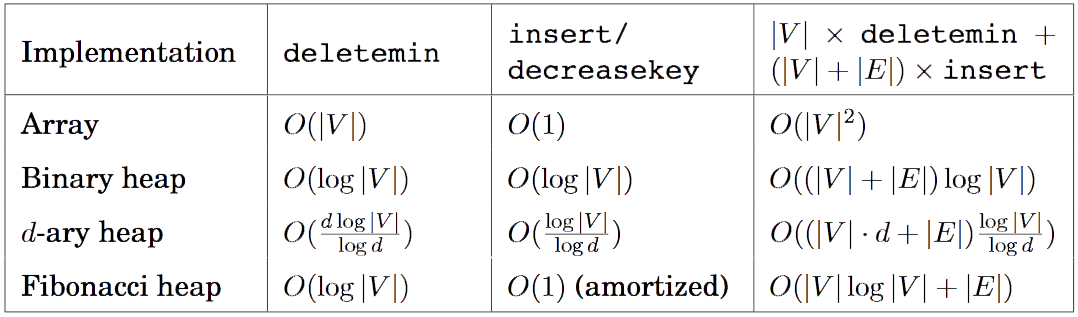
\includegraphics[scale=.2]{heaps.png}




% You can even have references
\rule{0.3\linewidth}{0.25pt}
\scriptsize
\bibliographystyle{abstract}
\bibliography{refFile}
\end{multicols}
\end{document}
